\chapter{Braille}

\section{Historia}
El sistema Braille es un m\'etodo utilizado por personas ciegas para leer y 
escribir. Fue ideado en 1821 por el franc\'es \emph{Louis
Braille}\footnote{V\'ease - \url{http://es.wikipedia.org/wiki/Luis_Braille}}
Se basa en un m\'etodo de comunicaci\'on desarrollado y perfeccionado por 
\emph{Charles Barbier}\footnote{V\'ease -
\url{http://en.wikipedia.org/wiki/Charles_Barbier}}, en respuesta a la demanda
de Napole\'on, de un c\'odigo que los soldados pudieran usar para comunicarse
en silencio y sin luz en la noche.
Se lo llam\'o \emph{Night writing}\footnote{V\'ease -
\url{http://en.wikipedia.org/wiki/Night_writing}}. El sistema de Barbier era
demasiado complejo para los soldados de aprender, y fue rechazada por los
militares. 
En 1821, Barbier, visit\'o el Instituto Nacional para Ciegos, en Par\'is, donde
conoci\'o a \emph{Louis Braille}, qui\'en identific\'o el mayor defecto del
c\'odigo: el dedo de la mano humana no puede abarcar todo el s\'imbolo sin
moverse, y as\'i no puede pasar r\'apidamente de un s\'imbolo a otro.
Su modificaci\'on fue utilizar una celda de 6 puntos (el sistema Braille) que 
revolucion\'o la comunicaci\'on escrita de los ciegos.
Cada c\'elula (o celda) braille o car\'acter se compone de seis posiciones de 
puntos, dispuestos en un rect\'angulo que contiene dos columnas de tres puntos
cada uno. Un punto puede ser colocado en alguna de las seis posiciones para
formar sesenta y cuatro ($2^{6}$) permutaciones, incluido el arreglo de puntos
que no se coloca. Una permutaci\'on puede ser descrita nombrando las posiciones
en que se disponen los puntos: Las posiciones est\'an universalmente numerados
de 1 a 3, de arriba a abajo, a la izquierda, y 4 a 6, de arriba a abajo, a la
derecha como se muestra en la figura \ref{fig:braille_cell}.

\clearpage
% http://es.wikipedia.org/wiki/Archivo:Brailleschrift_06_KMJ.svg
\begin{figure}[htp]
\centering
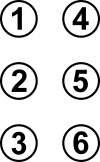
\includegraphics[scale=0.6]{./img/braille_cell.png}
\caption{Celda braille.}
\label{fig:braille_cell}
\end{figure}
\label{cap:braille_cell}

%%%%%%%%%%%%%%%%%%%
\section{T\'ecnica}
%%%%%%%%%%%%%%%%%%%
%
Las l\'ineas horizontales de texto en Braille est\'an separados por un espacio
a fin de que los puntos de una l\'inea puede ser diferenciada de la de texto
en braille por encima y por debajo. La puntuaci\'on est\'a representada por su
propio conjunto de caracteres \'unico. No existe una estandarizaci\'on
rigurosa para las distancias o medidas entre los puntos de las celdas braille,
aunque si se ha generado un est\'andar impl\'icito como muestra la figura
\ref{fig:distance_dots_braille}.


% http://www.wikilearning.com/monografia/abcsound-marco_teorico_1_parte/5508-9
\begin{figure}[htp]
\centering
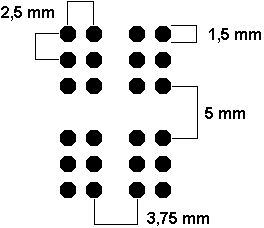
\includegraphics[scale=0.6]{./img/distance_dots_braille.png}
\caption{Medidas de las celdas braille.}
\label{fig:distance_dots_braille}
\end{figure}

La combinaci\'on de estos puntos generan el alfabeto braille y todos los
s\'imbolos, como se muestra en la tabla \ref{tab:alfabeto_braille}.

\begin{table}[htp]
\begin{center}
	\enskip \enskip
	\begin{tabular}[t]{r|l}
	\hline
		\braille{a} & a \\
		\braille{b} & b \\
		\braille{c} & c \\
		\braille{d} & d \\
		\braille{e} & e \\
		\braille{f} & f \\
		\braille{g} & g \\
		\braille{h} & h \\
		\braille{i} & i \\
		\braille{j} & j \\
		\braille{k} & k \\
		\braille{l} & l \\
		\braille{m} & m \\
	\hline
	\end{tabular}
	\enskip \enskip
	\enskip \enskip
	\begin{tabular}[t]{r|l}
	\hline
		\braille{n} & n \\
		\braillebox{12456} & \~n \\
		\braille{o} & o \\
		\braille{p} & p \\
		\braille{q} & q \\
		\braille{r} & r \\
		\braille{s} & s \\
		\braille{t} & t \\
		\braille{u} & u \\
		\braille{v} & v \\
		\braille{w} & w \\
		\braille{x} & x \\
		\braille{y} & y \\
		\braille{z} & z \\
	\hline
	\end{tabular}
	\enskip \enskip
	\enskip \enskip
	\begin{tabular}[t]{r|l}
	\hline
		\braillebox{12356} & \'a \\
		\braillebox{2346} & \'e \\
		\braillebox{34} & \'i \\
		\braillebox{346} & \'o \\
		\braillebox{23456} & \'u \\
		\braille{,} & , \\
		\braille{;} & ; \\
		\braille{:} & : \\
		\braillebox{3} & . \\
		\braille{!} & ! \\
		\braillebox{126} & ( \\
		\braillebox{345} & ) \\
		\braillebox{35} & *	\\
		\braillebox{25} & ?	\\
		\braillebox{236} & '' \\
	\hline
	\end{tabular}
	\enskip \enskip
\end{center}
\caption{Alfabeto castellano braille.}
\label{tab:alfabeto_braille}
\end{table}


Debido a la limitaci\'on que impone la reducida cantidad de combinaciones que
pueden generarse con \'este sistema de seis puntos, \emph{Louis Braille}
propuso reservar algunas combinaciones\footnote{\'Estos s\'imbolos suelen
variar dependiendo del idioma.} que, actuando como prefijos o sufijos y en
contexto, pueden cambiar el significado de los s\'imbolos adyacentes.\
Los ejemplos m\'as importantes son los de las letras may\'usculas (ver tabla
\ref{tab:braille_capital}) y la de los n\'umeros (ver tabla
\ref{tab:braille_numbers}). 

\begin{table}[htp]
\begin{center}
	\enskip \enskip
	\begin{tabular}[t]{r|l}
	\hline
		\braillebox{46} \braille{a} & A \\
		\braillebox{46} \braille{b} & B \\
		\braillebox{46} \braille{c} & C \\
		\braillebox{46} \braille{d} & D \\
		\braillebox{46} \braille{e} & E \\
		...							& ... \\
	\hline
	\end{tabular}
	\enskip \enskip	
\end{center}
\caption{May\'usculas braille.}
\label{tab:braille_capital}
\end{table}


\begin{table}[htp]
\begin{center}
	\enskip \enskip
	\begin{tabular}[t]{r|l}
	\hline
		\braillebox{3456} \braille{a} & 1 \\
		\braillebox{3456} \braille{b} & 2 \\
		\braillebox{3456} \braille{c} & 3 \\
		\braillebox{3456} \braille{d} & 4 \\
		\braillebox{3456} \braille{e} & 5 \\
		\braillebox{3456} \braille{f} & 6 \\
		\braillebox{3456} \braille{g} & 7 \\
		\braillebox{3456} \braille{h} & 8 \\
		\braillebox{3456} \braille{i} & 9 \\
		\braillebox{3456} \braille{j} & 0 \\
	\hline
	\end{tabular}
	\enskip \enskip	
\end{center}
\caption{N\'umeros braille.}
\label{tab:braille_numbers}
\end{table}

\newpage
Existen tres tipos de transcripci\'on \emph{braille}, conocidos como ``Grado
1'', ``Grado 2'' y ``Grado 3''. El \emph{braille} de grado 1, es el ideado por
\emph{Louis Braille} y considerado oficial\footnote{Esto depende
exclusivamente del idioma y los pa\'ises} en la mayor\'ia de los pa\'ises.\
Los grados 2 y 3 son conocidos como \emph{estenotopia}\footnote{V\'ease -
\url{http://es.wikipedia.org/wiki/Estenotipia}} y tienen como finalidad
economizar la cantidad de caracteres usados.\
Un ejemplo de \'esto es el usar un solo s\'imbolo de n\'umero cuando lo que
continua es todo un n\'umero como se ve a continuaci\'on:\\

\begin{center}
\braillebox{3456} \braille{a} \braille{b} \braille{c}\\
\begin{scriptsize}(num)\end{scriptsize} 1 \,  2  \, 3\\
\end{center}

O por ejemplo si se quiere hacer saber que toda la palabra siguiente se
encuentra en may\'uscula se anteponen dos s\'imbolos de may\'uscula como se ve
a
continuaci\'on:\\

\begin{center}
\braillebox{46} \braillebox{46} \braille{h} \braille{o} \braille{l}
\braille{a}\\
\begin{scriptsize}(may)(may)\end{scriptsize} H \, O \, L \, A\\
\end{center}

%%%%%%%%%%%%%%%%%%%%%%%%%%%%%%%%%%%%%%%%%%%%%%%%%%%%%%%%%%%%%%%%%%%%%%%%%%%%%%
%%%%%%%%%%%%%%%%%%%%%%%%%%%%%%%%%%%%%%%%%%%%%%%%%%%%%%%%%%%%%%%%%%%%%%%%%%%%%%
\newpage
\section{Braille escrito}
%
Como se explic\'o en la secci\'on anterior, el sistema braille escrito consta
de celdas de dos columnas de tres puntos, cada uno de los cuales puede estar
en relieve de la superficie en la que se est\'a escribiendo. Es de imaginarse
que existen muchas maneras de lograr esto. A continuaci\'on se explican los
m\'etodos m\'as usados.

\subsection{Regleta/pauta y punz\'on} 
%
Este m\'etodo es uno de los m\'as usados y quiz\'a uno de los m\'as
econ\'omicos.
Consta de dos plantillas de alg\'un material firme\footnote{Normalmente de
pl\'astico o aluminio} unidas en un extremo mediante una bisagra. Una de las
plantillas posee una matriz de celdas vac\'ias con separaciones est\'andar
entre
ellas, la otra posee una matriz de celdas con huecos c\'oncavos siguiendo el
est\'andar braille. Esta \emph{regleta} se alimenta con papel\footnote{Este
papel si bien no es necesario que sea especial, se usa alg\'un tipo de papel
grueso donde se puedan marcar puntos en relieve sin perforarlo.} entre ambas
plantillas, permitiendo luego, mediante un punz\'on de mano, ir marcando el
relieve de los puntos correspondientes a la letra braille que se desea
escribir. La figura \ref{fig:Slate_and_Stylus_3} muestra tres
tipos de regletas y dos punzones.

% http://upload.wikimedia.org/wikipedia/commons/e/e9/Slate_and_Stylus_3.jpg
\begin{figure}[htp]
\centering
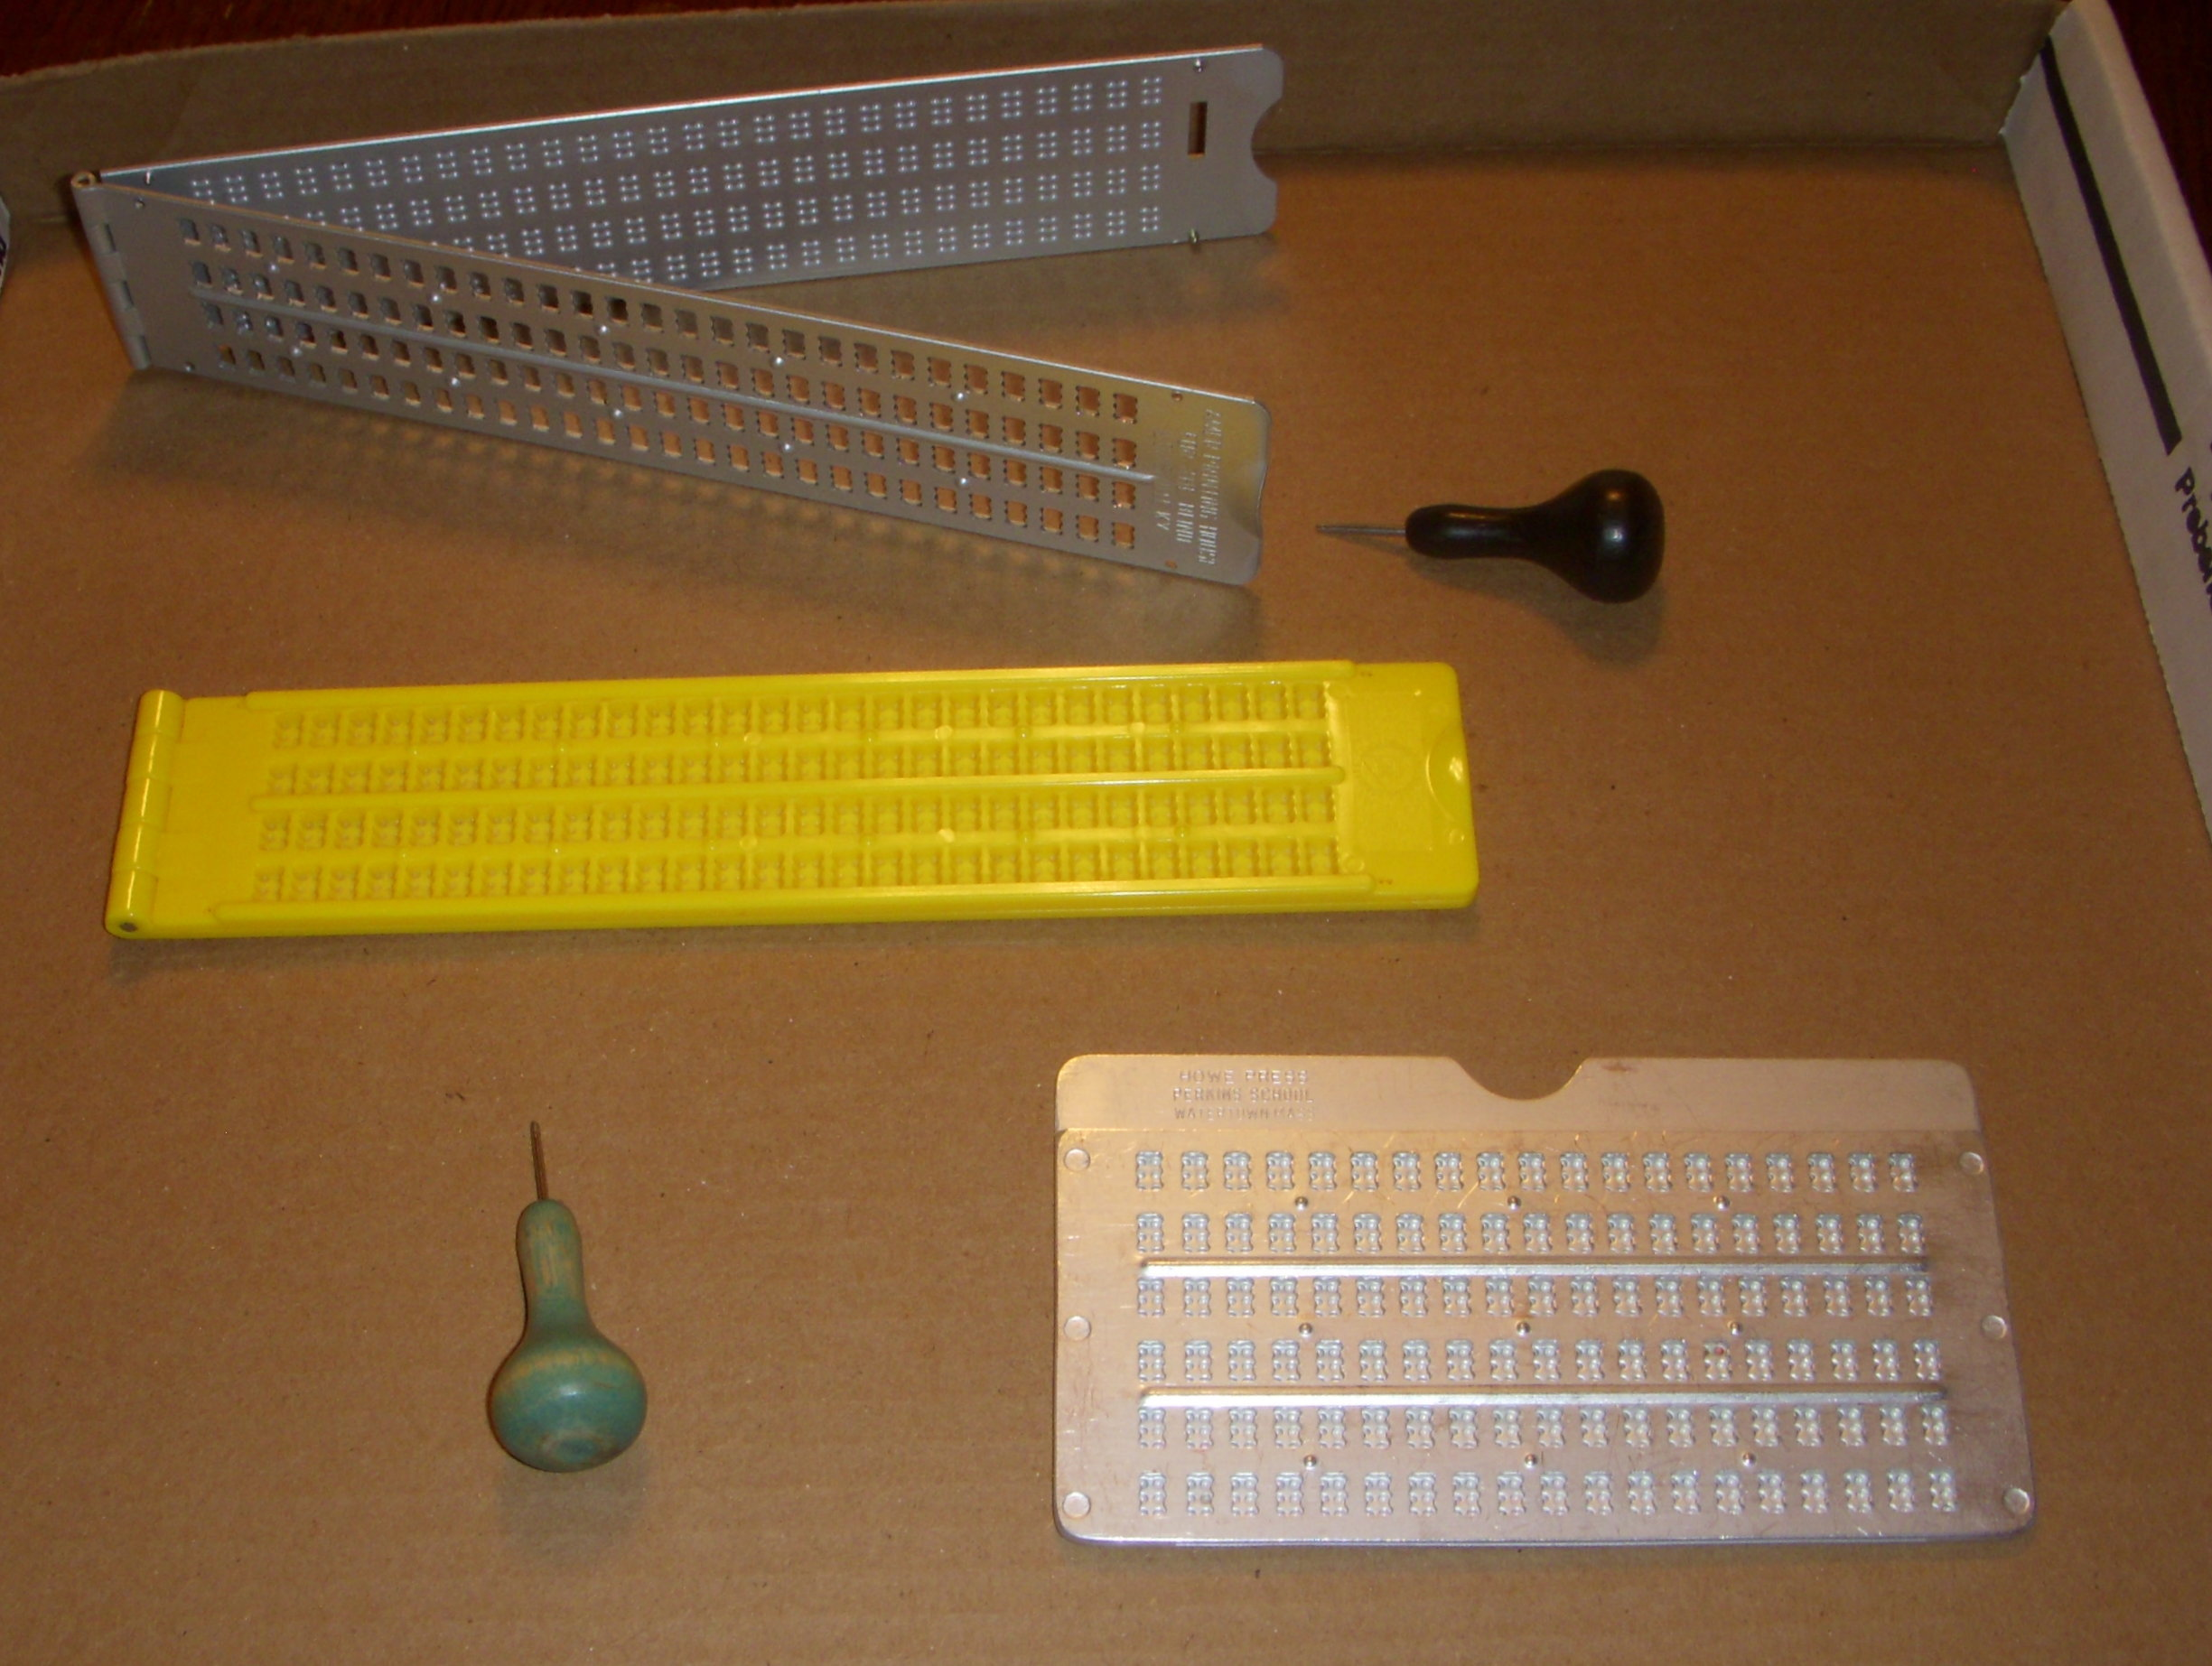
\includegraphics[width=12cm]{./img/Slate_and_Stylus_3.png}
\caption{Regletas y punzones para escritura braille.}
\label{fig:Slate_and_Stylus_3}
\end{figure}

Las principales desventajas de este m\'etodo, es que requiere que la persona
que escribe este muy capacitada y piense al rev\'es\footnote{Esto se debe a que
en las regletas las celdas se escriben del lado opuesto a donde se leer\'an}
mientras lo hace, adem\'as de que se obtienen muy pocos caracteres por minuto.

\subsection{Maquina de escribir braille}
%
En 1892 Frank Haven Hall
%\footnote{V\'ease - \url{
%http://books.google.com/books?id=u4uzPlgcWpsC&pg=PA452&lpg=PA452&dq=Frank+Have
%n+Hall&source=bl&ots=Xf_e354ZC9&sig=2T51O8wSR92Vj1tWHBtySCBU0Bg&hl=es&ei=eClWS
%qyAAcuwlAeC5ujcAg&sa=X&oi=book_result&ct=result&resnum=9}} 
invent\'o una maquina
compleja completamente mec\'anica pero de funcionamiento muy sencillo para la
escritura braille.\\

Hasta el d\'ia de hoy las actuales maquinas de escribir braille se basan en los
mismos principios de funcionamientos que aquella que inven\'o Frank Haven Hall,
pero la tecnolog\'ia de fabricaci\'on se basa materiales m\'as livianos y
resistentes que los de aquella \'epoca. \\

El mecanismo consiste de una parte m\'ovil con movimientos horizontales donde
se
fija el papel el cual puede a se vez desplazarse hacia arriba o hacia abajo
como en las maquinas de escribir comunes. Posee seis teclas que mueven un
juego de v\'astagos que a su vez activan una serie de punz\'ones que marcan la
hoja. Estas seis teclas permiten escribir (o impactar) un caracter braille a
la vez, y luego existe una s\'eptima tecla\footnote{Esto seria similar a la
barra espaciadora de las maquinas de escribir convencionales.} que se encarga
de
desplazar la hoja hacia un lado permitiendo as\'i escribir un caracter nuevo.\\

Se puede ver en la figura \ref{fig:hallbraille-03} la maquina original
inventada por Frank Haven Hall, y en la figura
\ref{fig:ng_perkinsaph_brailler} se muestra un modelo nuevo que se puede
encontrar actualmente en el mercado.

% http://www.typewriter.be/hallbraille.htm
\begin{figure}[htp]
\centering
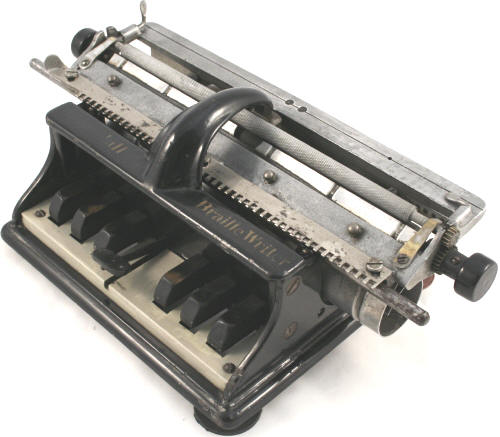
\includegraphics[width=10cm]{./img/hallbraille-03.png}
\caption{Primera maquina de escribir braille inventada por Frank Haven Hall
en 1892.}
\label{fig:hallbraille-03}
\end{figure}

%https://secure2.convio.net/psb/site/Ecommerce/1079514097?VIEW_PRODUCT=true&pro
%d uct_id=2041&store_id=1101
\begin{figure}[htp]
\centering
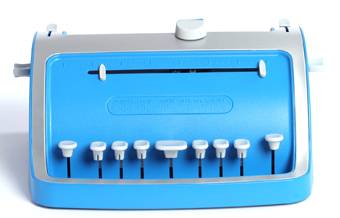
\includegraphics[width=10cm]{./img/ng_perkinsaph_brailler.png}
\caption{Maquina de escribir braille actual del mercado.}
\label{fig:ng_perkinsaph_brailler}
\end{figure}

Estas maquinas, al igual que la regleta y el punz\'on, requieren una persona
con conocimientos y pr\'actica para su uso, pero poseen la ventaja de que se
pueden lograr una mayor cantidad de caracteres por minuto. De hecho cuando
Frank Haven Hall present\'o su invento, impresion\'o a la audiencia con una
velocidad de 58 palabras por minuto.



\subsection{Impresoras braille}
%
La primera\footnote{V\'ease - \url{http://www.duxburysystems.com/bthist.asp}}
impresora braille\footnote{El t\'ermino correcto es \emph{impactadora} debido a
que proviene del ingl\'es \emph{embosser}} para papel normal fue fabricada en
el Instituto de Tecnolog\'ia de Masachusset (\emph{MIT - Massachusetts
Institute
of Technology})\footnote{V\'ease - \url{http://web.mit.edu/}} a finales de la
d\'ecada de los 60 y se llam\'o \emph{BrailleEmboss} cuyo dise\~no estuvo a
cargo
de George Dalrymple\footnote{V\'ease - \url{
http://www.ll.mit.edu/Retirees/Picnic05/index_04.html}}.\\

Esta impresora formaba parte de un proyecto m\'as grande llamado
DOTSYS\footnote{V\'ease - \url{http://www.dpawson.co.uk/braille/braille.html}}
cuyo objetivo era crear un programa para traducir texto en ingl\'es a braille
ingl\'es est\'andar. 
Ten\'ia la capacidad de producir una p\'agina braille de 38
celdas de ancho por 25 de largo cada 1.6 a 2 minutos.
Soportaba diversos m\'etodos de entrada de dato, entre ellos tarjetas
perforadas, teclado o cintas de teletipo\footnote{V\'ease -
\url{http://es.wikipedia.org/wiki/Teletipo}}. Debido al car\'acter mayormente
investigativo de este proyecto solo se fabricaron una veintena de estas
impresoras y su costo de producci\'on es desconocido.\\

Existen actualmente en el mercado una amplia variedad de impresoras braille
para cubrir la mayor\'ia de las necesidades de los usuarios, desde impresoras
personales hasta impresoras para grandes niveles de producci\'on, con
velocidades de impresi\'on desde 10 hasta 400 caracteres por segundo y
precios desde 3200 hasta m\'as de 30000 dolares.\\

Las impresoras braille com\'unmente se especifican seg\'un:

\begin{itemize}
 \item Velocidad medida en CPS (caracteres por segundo)
 \item Tama\~no
 \item Peso
 \item Nivel de ruido en dB
 \item Tipo de papel que soporta
 \item Consumo de potencia el\'ectrica en estado inactivo
 \item Consumo de potencia el\'ectrica durante funcionamiento
\end{itemize}

Debido a su principio de funcionamiento de impresi\'on por impacto el nivel de
ruido es una de las caracter\'isticas m\'as importantes al igual que su peso
proveniente mayormente de la fuente y los mecanismos de impacto.\\

La caracter\'istica m\'as atrayente de las impresoras braille es que pueden ser
utilizadas por personas con muy poco conocimiento, ya que la parte t\'ecnica
del braille es resuelta enteramente por software, entonces basta solo con
escribir el texto que se desea imprimir en el idioma deseado y luego mediante
software este es traducido y enviado a la impresora quien se encargara de
imprimirlo.

\subsubsection{Funcionamiento}
%
La mayor\'ia de las impresoras braille del mercado tienen un funcionamiento
similar. Se escribe el texto que se desea imprimir en un editor de texto, ya
sea com\'un o bien uno provisto por el fabricante, una vez que se ha terminado
el texto se necesita generar una especie de vista preliminar donde se pueden
observar las modificaciones que agragar\'a el programa para cumplir con las
limitaciones del braille usando una tipograf\'ia braille. Luego el documento se
\emph{traduce} a un metalenguaje que contiene tanto el texto como caracteres
adicionales inherentes al braille pero con una codificaci\'on particular que
interpretar\'a la impresora. La informaci\'on codificada puede ser guardada
para una posterior impresi\'on o directamente puede enviarse a imprimir.\\

La forma en la que las impresoras marcan el papel depende, entre otras cosas,
del fabricante, el mercado que cubre, la tecnolog\'ia usada, la precisi\'on, y
otros factores.  
No obstante pueden diferenciarse dos grandes soluciones entre las m\'as
usadas; punz\'on \'unico desplazante y m\'ultiples punzones desplazantes.\\

En la actualidad la mayor\'ia de las impresoras braille hacen uso del mecanismo
de m\'ultiples punzones desplazantes, ya que \'este m\'etodo permite una mayor
velocidad de impresi\'on (caracteres por segundo), pero como contrapartida esta
tecnolog\'ia encarece enormemente el producto, ya que los punzones se fabrican
a
medida y son de alta precisi\'on. En la figura
\ref{fig:embosser_index_multiple_hammers} se puede observar un cabezal de trece
punzones que es usado por las impresoras braille del fabricante \emph{Index
Braille}\footnote{V\'ease - \url{http://www.indexbraille.com/}}.

%http://www.cascade.fi/getmedia/642f2c5b-0882-4401-ab37-d3a305b33d0b/Embosser_h
%ammer_adjustment_080512_640x360.mp4?preview=1&width=828&height=466
\begin{figure}[htp]
\centering
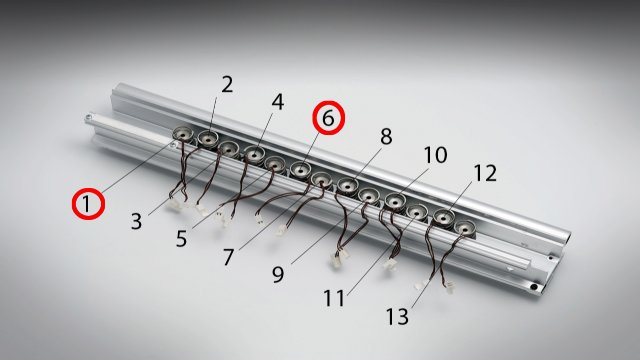
\includegraphics[width=12cm]{./img/embosser_index_multiple_hammers.png}
\caption{M\'ultiples punzones desplazantes.}
\label{fig:embosser_index_multiple_hammers}
\end{figure}

El cabezal solo necesita un peque\~no desplazamiento horizontal para cubrir el
ancho completo de la hoja y generar una secuencia continua de tres filas de
puntos.\'Este mecanismo tambi\'en permite la impresi\'on de braille en ambos
lados de la hoja, intercalando punzones c\'oncavos y convexos como se aprecia
en la figura \ref{fig:embosser_index_cut_hammers}.

% http://epubl.luth.se/1402-1617/2006/215/LTU-EX-06215-SE.pdf
\begin{figure}[htp]
\centering
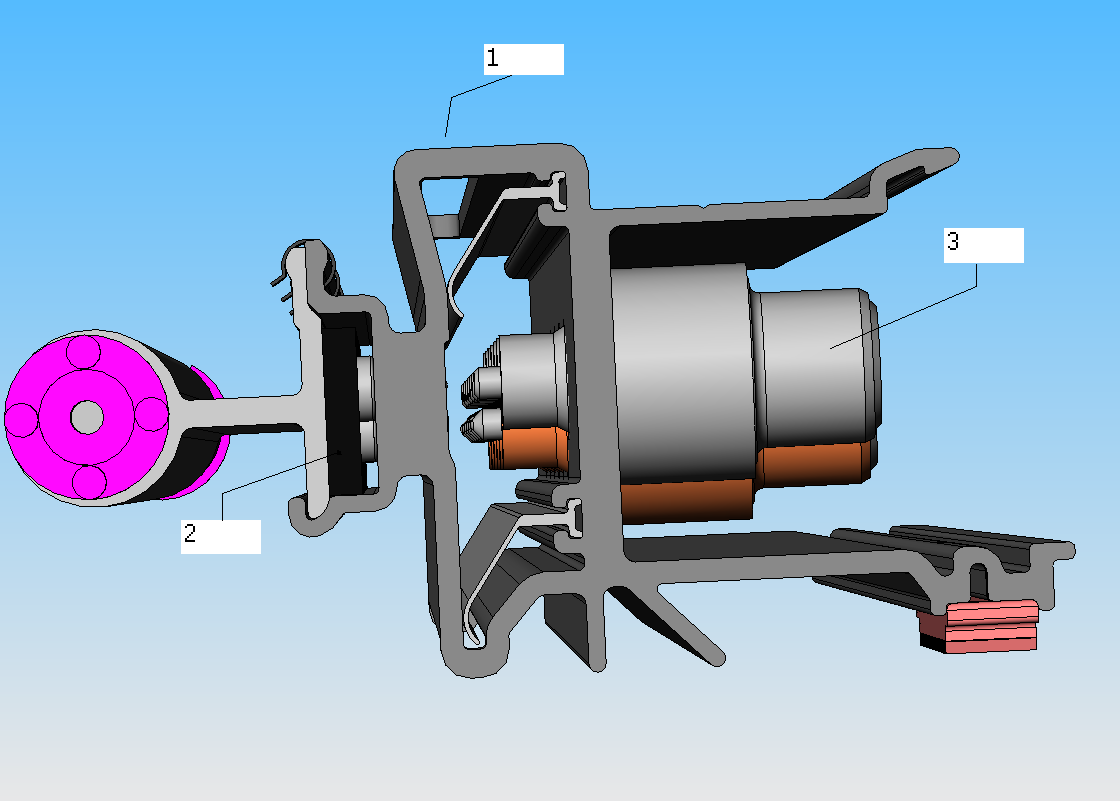
\includegraphics[width=10cm]{./img/embosser_index_cut_hammers.png}
\caption{Corte cabezal IndexBraille. 1 - Alimentaci\'on de papel, 2 - Yunque de
goma, 3 - Punz\'on o martillo}
\label{fig:embosser_index_cut_hammers}
\end{figure}

Los punzones grises poseen punta convexa, mientras que los marrones poseen
punta c\'oncava. Fijos al yunque de goma se encuentra una matriz de punzones
que encastran perfectamente con sus respectivos punzones m\'oviles, y es entre
\'estos que el papel es impactado gener\'andose el relieve hacia un lado o
hacia
el otro. \\

%Existen varios mecanismos distintos que han ido evolucionando con
El mecanismo de cabezal con un \'unico punz\'on desplazante no es muy usado
en la actualidad debido a que es muy lento, sin embargo es una de las
soluciones m\'as econ\'omicas. Consiste en un cabezal m\'ovil con un \'unico
punz\'on, el cual se desplaza a lo ancho de la hoja golpeando cada vez que se
desea marcar un punto. Un esquema de este mecanismo se puede ver en la figura 

%
% Agregar imagen de cabezal con un unico punzon !!!!!!!!!!!!!!!!!!!!!!!!!!!!!!
%

La sencillez de este mecanismo le otorga tanto robustez como versatilidad,
junto a un dise\~no simple de bajo costo de producci\'on y mantenimiento.Todas
estas caracter\'isticas hacen de este sistema el ideal para implementar un
dispositivo econ\'onmico y sencillo, raz\'on por la cual sera el usado en
este trabajo.